% !TEX TS-program = pdflatex
% !TEX encoding = UTF-8 Unicode

% This is a simple template for a LaTeX document using the "article" class.
% See "book", "report", "letter" for other types of document.

\documentclass[11pt]{article} % use larger type; default would be 10pt

\usepackage[utf8]{inputenc} % set input encoding (not needed with XeLaTeX)

%%% Examples of Article customizations
% These packages are optional, depending whether you want the features they provide.
% See the LaTeX Companion or other references for full information.

%%% PAGE DIMENSIONS
\usepackage{geometry} % to change the page dimensions
\geometry{a4paper} % or letterpaper (US) or a5paper or....
% \geometry{margin=2in} % for example, change the margins to 2 inches all round
% \geometry{landscape} % set up the page for landscape
%   read geometry.pdf for detailed page layout information

\usepackage{graphicx} % support the \includegraphics command and options

% \usepackage[parfill]{parskip} % Activate to begin paragraphs with an empty line rather than an indent

%%% PACKAGES
\usepackage{booktabs} % for much better looking tables
\usepackage{array} % for better arrays (eg matrices) in maths
\usepackage{paralist} % very flexible & customisable lists (eg. enumerate/itemize, etc.)
\usepackage{verbatim} % adds environment for commenting out blocks of text & for better verbatim
\usepackage{subfig} % make it possible to include more than one captioned figure/table in a single float
% These packages are all incorporated in the memoir class to one degree or another...

%%% HEADERS & FOOTERS
\usepackage{fancyhdr} % This should be set AFTER setting up the page geometry
\pagestyle{fancy} % options: empty , plain , fancy
\renewcommand{\headrulewidth}{0pt} % customise the layout...
\lhead{}\chead{}\rhead{}
\lfoot{}\cfoot{\thepage}\rfoot{}

%%% SECTION TITLE APPEARANCE
\usepackage{sectsty}
\allsectionsfont{\sffamily\mdseries\upshape} % (See the fntguide.pdf for font help)
% (This matches ConTeXt defaults)

%%% ToC (table of contents) APPEARANCE
\usepackage[nottoc,notlof,notlot]{tocbibind} % Put the bibliography in the ToC
\usepackage[titles,subfigure]{tocloft} % Alter the style of the Table of Contents
\renewcommand{\cftsecfont}{\rmfamily\mdseries\upshape}
\renewcommand{\cftsecpagefont}{\rmfamily\mdseries\upshape} % No bold!


\usepackage{hyperref}
\hypersetup{
    colorlinks=true,
    linkcolor=blue,
    filecolor=magenta,      
    urlcolor=cyan,
}
%%% END Article customizations

%%% The "real" document content comes below...

\title{ID2205 - Project Specification}
\author{Student: Leon Fernandez\\Supervisor: Peng Wang}
\date{} % Activate to display a given date or no date (if empty),
         % otherwise the current date is printed 

\begin{document}
\maketitle

\section*{Overview}
At its core the project consists of building a web-based development environment (DE) for the graphical programming language DMDL [1]. Documentation and version control will be done using appropriate software (such as JSDoc and Git [2], [3]) and the results will be presented orally, in a written report and in a short screencast demonstation.

\section*{Workflow}
The DE will be built using standard web technologies such as JavaScript, CSS and HTML, [4], [5], [6], and it should feature a drag-and-drop type interface similar to LabVIEW or Simulink [7], [8]. An existing set of graphics exists for the language's blocks, an example of which can be seen in Figure \ref{fig:block}. These can be used as a base for the blocks in the DE. By adding, for example, dropdown menus and text bars to the blocks the user will be able to alter the behavior of the blocks, such as changing values of timers. 

Since the DE is just a small part of a larger project, it is of great importance that the code is well-documented and maintainable so that it can be integrated into a larger ecosystem and so that future features can easily be added. Some of these features are already known and the project should make an effort to facilitate their implementations. For instance, one such feature is the ability to interface with Gnu Radio [9].

A traditional Model-View-Controller [10] design pattern will be used for the code architecture. The ''Model''-component should be written in such a way that future developers can easily add features such as being able to program Software Defined Radios from the DE or interface with Gnu Radio, as previously mentioned. This is illustrated in Figure \ref{fig:MVC}.

\newpage
\section*{Grading Guidelines}

\textit{I borrowed these guidelines from the course DH2641. I think we can use these as a base for our own guidelines if Christian wants to have a structured grading scale. Link to the course web for DH2641 here:\\
\url{https://www.kth.se/social/course/DH2641/subgroup/vt-2015-iprog14/page/final-project-5/}}
\\\\
Working project with high usability and good architecture: A\\
Working project with high usability but architectural issues: B\\
Working project with good architecture and usability problems: B\\
Working project with usability problems and architectural issues (or major usability problems): C\\
Project with minor bugs but good architecture: D\\
Project with minor bugs or achitectural flaws: E\\
Project with major bugs or major architectural flaws: Fx\\

\section*{Expected Outcome}
The expected outcome of the project is:\\
- Well-documented and version controlled source code for the DE\\
- An oral presentation and demonstration of the DE\\
- A screencast showing off the basic features of the DE\\
- A written technical report

\section*{References}
[1] Peng Wang's Github \\
{[2]} JSDoc Website \\
{[3]} Git Website \\
{[4]} JavaScript Website \\
{[5]} CSS Website \\
{[6]} HTML Website \\
{[7]} LabVIEW Website \\
{[8]} Simulink Website
{[9]} Gnu Radio Website \\
{[10]} Model-View-Controller Description

\begin{figure}[h]
\centering
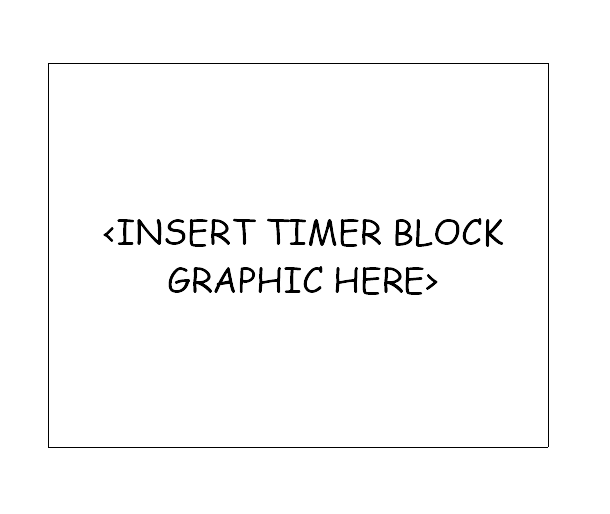
\includegraphics[scale=0.4]{block}
\caption{An example of what a timer block might look like.}
\label{fig:block}
\end{figure}

\begin{figure}[h]
\centering
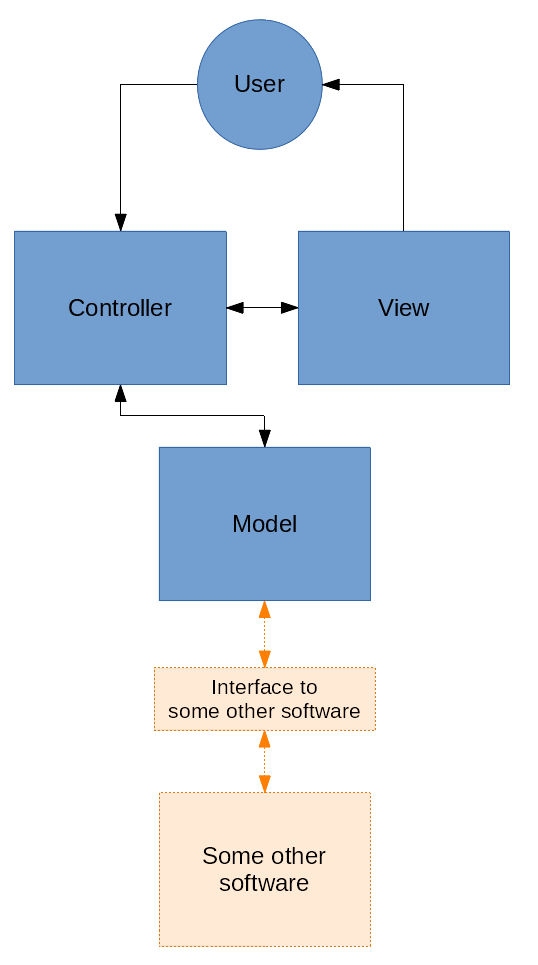
\includegraphics[scale=0.5]{MVC}
\caption{An illustration of the code architecture.}
\label{fig:MVC}
\end{figure}

\end{document}
